\documentclass[a4paper, 10pt]{article}
\usepackage{helvet}
\renewcommand{\familydefault}{\sfdefault}
\usepackage{pgf}
\usepackage{eurosym}
\usepackage{graphicx}
\usepackage{wasysym}
\usepackage{hyperref}
\usepackage{listings}
\usepackage{pxfonts}
\usepackage{verbatim}
\usepackage{color}
\usepackage{xcolor}
\usepackage{wrapfig}
\usepackage{enumitem}
\usepackage{booktabs}
\usepackage{gensymb}
\usepackage{tabularx}
\usepackage{currfile}

\hypersetup{
    bookmarks=true,         % show bookmarks bar?
    unicode=true,          % non-Latin characters in Acrobat’s bookmarks
    pdftoolbar=true,        % show Acrobat’s toolbar?
    pdfmenubar=true,        % show Acrobat’s menu?
    pdffitwindow=true,     % window fit to page when opened
    pdftitle={Assessments},    % title
    pdfauthor={Paul Vesey},     % author
    pdfsubject={Building Information Modelling },   % subject of the document
    pdfcreator={},   % creator of the document
    pdfproducer={xelatex}, % producer of the document
    pdfkeywords={'Graphics' }, % list of keywords
    pdfnewwindow=true,      % links in new PDF window
    colorlinks=true,       % false: boxed links; true: colored links
    linkcolor=violet,          % color of internal links (change box color with linkbordercolor)
    citecolor=magenta,        % color of links to bibliography
    filecolor=red,      % color of file links
    urlcolor=blue           % color of external links
}

\setlength\parindent{0pt}
\begin{document}

\lstset{language=HTML,
				basicstyle=\small,
				breaklines=true,
        numbers=left,
        numberstyle=\tiny,
        showstringspaces=false,
        aboveskip=-20pt,
        frame=leftline
        }


\begin{figure}
	\centering
	\includegraphics[width=0.5\linewidth]{./img/TUSlogo}
\end{figure}


\begin{tabularx}{\textwidth}{ |l|X| }
	\hline
	
	\textbf{Subject:} & Health \& Safety IT\\
	\textbf{Course:} & BSc in Construction Health \& Safety\\
	\textbf{Session:} & Autumn 2021\\
	\textbf{Lecturer:} & Paul Vesey \footnotesize{BEng, MIE, HDip}\\
	\textbf{Filename:} & \currfilebase\\
	\hline
\end{tabularx}

	
\part*{Assignment 3 (33\%) - Autodesk BIM360}

\begin{tabularx}{\textwidth}{ |X|X| }
	\hline
	\textbf{Issue Date:} & As stated on Moodle \\
	\hline 
	\textbf{Submission Date:}  & As stated on Moodle  \\
	\hline
\end{tabularx}


\section*{Assignment Outline}


In this assignment you will create a BIM360 Field Survey to capture a workplace audit.  The questions that are to be used are taken from \href{https://safetyculture.com/}{https://safetyculture.com/}, iAudior example survey.   Autodesk BIM360 is available at \href{https://docs.b360.autodesk.com/}{https://docs.b360.autodesk.com/}.


\section*{Background Information}

In a previous assignment, you created a digital survey using Microsoft Forms.  In this assignment you will also create a survey, but this time the survey will be integrated into Autodesk BIM360 and used in association with a Building Information Model.


\begin{figure}
	\centering
	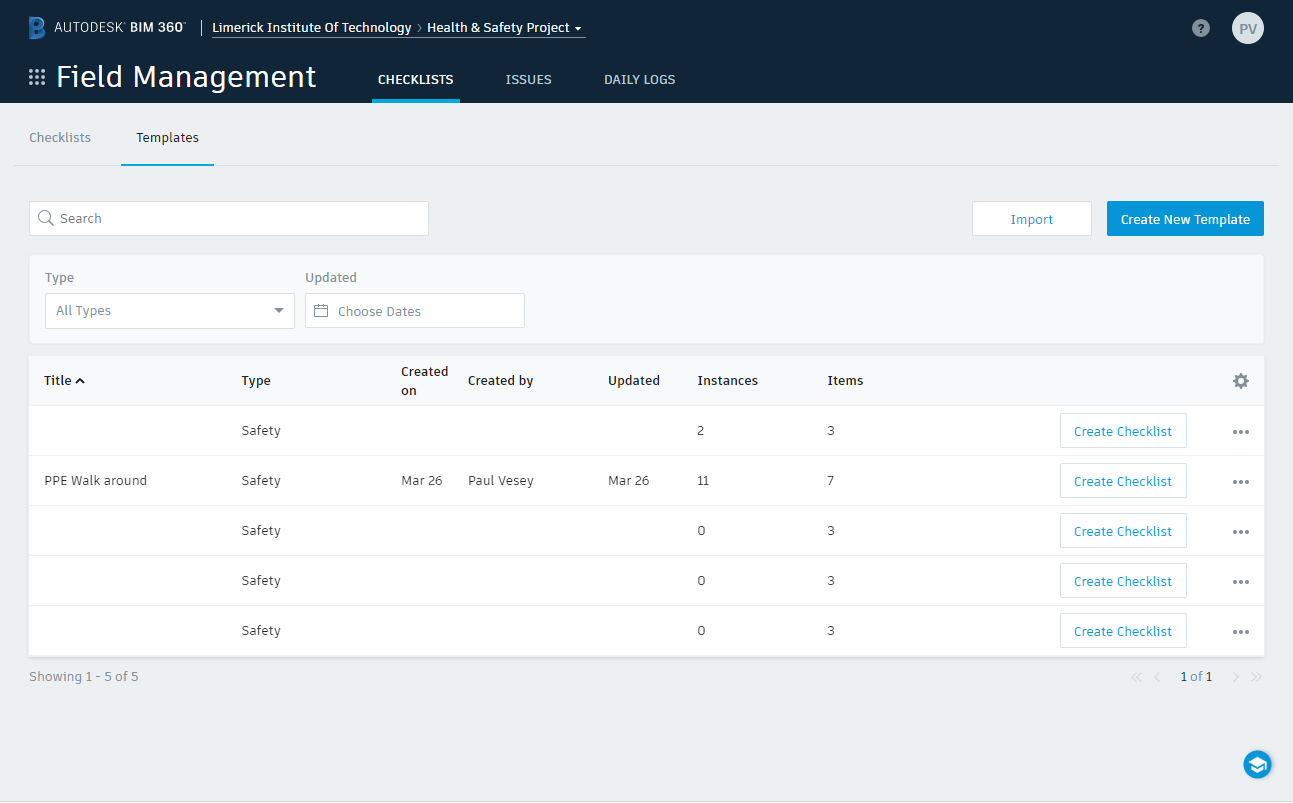
\includegraphics[width=1.0\linewidth]{./img/Template.png}
	\caption{BIM360 Checklist Template}
	\label{fig:BIM369ChecklistTemplate}
\end{figure}


\newpage
\section*{Layout \& Functionality}

The questions for the survey have been provided to you in the asset pack.  You are to implement as shown.  When you are testing the functionality of the survey on a smartphone should ensure that you have at least the following:

\begin{itemize}
	\item Photograph attached
	\item Annotated Photograph attached
	\item Voice Recognition used
	\item Issue Created
	\item Note Created
\end{itemize}

\section*{Testing}
You should ensure that your template is working as anticipated, including the functionality shown above.


\newpage
\section*{Checklists (x5)}
Group testing will not be implemented in this assignment.  Instead, it will be necessary for you to test your survey yourself prior to issuing to 5 of your classmates.  Each student is required to obtain 5 surveys from classmates as part of this assignment.


\section*{Submission}
This is a relatively complex submission, that will comprise many parts.  The parts are as follows:
\begin{enumerate}
	\item BIM360 Template (hosted on 'Health \& Safety Project' on BIM360)
	\item 5 Checklists completed by other students using the BIM360 Smartphone App
	\item 1000 word report on the creation and deployment of the BIM360 survey, including data analysis, app screenshots, and other items as may be required.  This document is to be a fully detailed report submitted in .pdf format only.
\end{enumerate}



\section*{Marking Scheme}
\begin{table}[h!]
	\begin{center}
		\begin{tabular}{p{8cm}  p{2cm} }
			\toprule
			\large{Element} & \large{Proportion} \\ 
			\cmidrule(r){1-1}\cmidrule(lr){2-2}
			BIM360 Field Template & 60\%\\
			Survey Deployments (x5) & 20\%\\
			Final Report & 20\%\\     
			\\ \bottomrule
		\end{tabular}
		\label{tbl:markSchemeAsmt3}
	\end{center}
\end{table}


\end{document}